\documentclass[12pt, a4paper]{article}

% ─── Packages ────────────────────────────────────────────────────────────────
\usepackage[utf8]{inputenc}
\usepackage[T1]{fontenc}
\usepackage{amsmath, amssymb, amsfonts}
\usepackage{graphicx}
\usepackage{booktabs}
\usepackage[numbers, sort&compress]{natbib}
\usepackage[colorlinks=true, linkcolor=blue!70!black, citecolor=blue!70!black, urlcolor=blue!60!black]{hyperref}
\usepackage{geometry}
\usepackage{enumitem}
\usepackage{xcolor}
\usepackage{tikz}
\usetikzlibrary{arrows.meta, positioning, shapes.geometric, fit, calc, backgrounds}
\usepackage{caption}
\usepackage{subcaption}
\usepackage{float}
\usepackage{fancyhdr}
\usepackage[most]{tcolorbox}

\geometry{margin=1in}

% ─── Header / Footer ────────────────────────────────────────────────────────
\pagestyle{fancy}
\fancyhf{}
\fancyhead[L]{\small\textit{Research Proposal: Metabolic Active Inference in Creatures 3}}
\fancyhead[R]{\small\thepage}
\renewcommand{\headrulewidth}{0.4pt}

% ─── Custom Commands ────────────────────────────────────────────────────────
\newcommand{\Hbio}{H_{\mathrm{bio}}}
\newcommand{\Rmig}{R_{\mathrm{mig}}}
\newcommand{\KL}{\mathrm{D_{KL}}}

% ─── Plain-Language Box Style ────────────────────────────────────────────────
\newtcolorbox{plainbox}[1][]{
  colback=blue!3!white,
  colframe=blue!40!black,
  coltitle=white,
  fonttitle=\small\bfseries,
  title={\raisebox{-1pt}{\small$\triangleright$}~In Plain English},
  boxrule=0.5pt,
  arc=2pt,
  left=6pt, right=6pt, top=4pt, bottom=4pt,
  fontupper=\small,
  #1
}

\newtcolorbox{analogybox}[1][]{
  colback=orange!4!white,
  colframe=orange!60!black,
  coltitle=white,
  fonttitle=\small\bfseries,
  title={\raisebox{-1pt}{\small$\approx$}~Analogy},
  boxrule=0.5pt,
  arc=2pt,
  left=6pt, right=6pt, top=4pt, bottom=4pt,
  fontupper=\small,
  #1
}

\newtcolorbox{glossarybox}[1][]{
  colback=green!3!white,
  colframe=green!50!black,
  boxrule=0.5pt,
  arc=2pt,
  left=6pt, right=6pt, top=4pt, bottom=4pt,
  fontupper=\small,
  #1
}

% ─── Title ───────────────────────────────────────────────────────────────────
\title{%
  \textbf{Thermodynamic Grounding of Neural Complexity:}\\[6pt]
  \large A Research Proposal for Metabolic Active Inference\\in \textit{Creatures 3}%
}
\author{%
  Cyril Sadovsky\\[2pt]
  \small Independent AI Researcher\\
  \small AE01.io --- Automate Everything\\[2pt]
  \small \texttt{cyril@ae01.io}
}
\date{July 2026}

% ═════════════════════════════════════════════════════════════════════════════
\begin{document}
\maketitle
\thispagestyle{fancy}

% ─── Plain Language Summary ──────────────────────────────────────────────────
\begin{tcolorbox}[
  colback=yellow!5!white,
  colframe=black!70,
  coltitle=black,
  fonttitle=\large\bfseries,
  title={Plain Language Summary},
  boxrule=1pt,
  arc=3pt,
  left=8pt, right=8pt, top=6pt, bottom=6pt,
]
\textbf{What is the problem?}
Today's AI systems like ChatGPT are incredibly capable, but they have no sense of \emph{cost}. They will use the same enormous amount of computing power whether the question is trivial or profound. Biological brains are different: every thought costs real energy. Your brain consumes about 20\% of all the calories you eat, even though it weighs only 2\% of your body. This energy cost is not a flaw---it forces your brain to be efficient, to prune unused connections, and to develop compact, effective representations of the world.

\medskip
\textbf{What are we testing?}
We take \textit{Creatures~3}, a 1998 artificial life game where virtual creatures called ``Norns'' have simulated brains, organs, and biochemistry. We modify the game engine so that every time a Norn's brain fires a neuron or rewires a connection, it costs the creature real metabolic energy (ATP---the same energy currency used by biological cells). We then ask: \emph{Does making thinking expensive force these artificial creatures to develop smarter, more efficient brains? And do creatures with ``expensive brains'' actually survive longer?}

\medskip
\textbf{How do we test it?}
We run 20 simulated trials: 10 where brain activity costs energy (treatment) and 10 where it does not (control). Each trial starts with 4 identical Norns and runs until the population goes extinct or 14 hours of simulated time passes. We record everything---brain activity, chemical levels, connection rewiring, births, and deaths---and compare the two groups.

\medskip
\textbf{Why does it matter?}
If making thinking expensive leads to more efficient brains and better survival, it suggests that the energy crisis facing modern AI (bigger models require exponentially more power) could be addressed not by adding more computing power, but by imposing the same kind of metabolic constraints that shaped biological intelligence over millions of years of evolution.
\end{tcolorbox}

\bigskip

% ─── Abstract ────────────────────────────────────────────────────────────────
\begin{abstract}
Modern large language models and artificial agents lack an underlying physiological homeostatic modulation system---a ``limbic gap'' that prevents continuous real-time learning and leads to energy-inefficient compute scaling. This research proposal specifies a controlled experiment that grounds the abstract information-theoretic complexity penalty of Karl Friston's Free Energy Principle (FEP) in a \emph{physical metabolic cost}: each neuron firing and each synaptic migration event in a \textit{Creatures~3} Norn brain deducts adenosine triphosphate (ATP) from the agent's biochemistry. Using the open-source Creatures~3 engine port with native in-engine telemetry, we test two hypotheses: (1)~that metabolic brain constraints force the emergence of sparse, high-efficiency synaptic networks, and (2)~that metabolically constrained agents exhibit superior survival and homeostatic stability across multiple generations. We propose a 2-condition between-subjects design (N=10 per condition), running each trial to population extinction or 3~million ticks, with Mann-Whitney~U tests as primary confirmatory analysis and Bayesian model comparison as supplementary analysis.
\end{abstract}

\medskip
\noindent\textbf{Keywords:} Free Energy Principle, Active Inference, Artificial Life, Metabolic Computing, Synaptic Plasticity, Creatures~3, Homeostasis, Limbic Gap

% ─── Key Terms Glossary ──────────────────────────────────────────────────────
\begin{glossarybox}
\textbf{Key Terms for Non-Specialist Readers}

\smallskip
\begin{description}[style=nextline, font=\small\bfseries, leftmargin=1.2cm, nosep, itemsep=3pt]
  \item[Norn] A virtual creature in the \textit{Creatures~3} game. Each Norn has its own brain, body chemistry, and DNA.
  \item[ATP] Adenosine triphosphate---the ``energy currency'' of cells. In both real biology and in the game, ATP powers cellular processes. When ATP runs low, the organism becomes fatigued.
  \item[Neuron] A brain cell that processes information. In the game, neurons are simplified digital units that ``fire'' (activate) when they receive enough input.
  \item[Synapse] A connection between two neurons. Information flows from one neuron to another through synapses. ``Synaptic weight'' describes how strong that connection is.
  \item[Synaptic Migration] When a brain connection is too weak to be useful, it disconnects and reattaches to a different neuron---like replumbing a pipe to a different outlet.
  \item[Homeostasis] The body's tendency to maintain stable internal conditions (temperature, hunger, energy). A Norn that maintains good homeostasis is healthy.
  \item[Entropy] A measure of disorder or unpredictability. Low entropy means stable and predictable; high entropy means chaotic and disordered.
  \item[Free Energy Principle (FEP)] A theory by neuroscientist Karl Friston proposing that all living things try to minimize ``surprise''---the gap between what they expect and what actually happens.
  \item[Pre-Registration] A public commitment to the design and analysis plan of an experiment \emph{before} running it, to ensure scientific transparency. A formal pre-registration for this study will be deposited on the Open Science Framework (OSF) prior to data collection.
  \item[Tick] One time step in the game simulation. The engine processes about 6 ticks per second at normal speed.
\end{description}
\end{glossarybox}

% ═════════════════════════════════════════════════════════════════════════════
\section{Introduction}
\label{sec:intro}

% ─── 1.1 The Limbic Gap ─────────────────────────────────────────────────────
\subsection{The Limbic Gap in Modern AI}

Imagine an employee who is brilliant at answering questions but has no sense of effort, fatigue, or cost. They will write a 10-page report whether you ask them a yes-or-no question or request a PhD thesis. They never learn to be concise, because being verbose doesn't tire them out. This is, in essence, the problem with modern AI.

Large Language Models (LLMs) like ChatGPT and Claude achieve remarkable performance on benchmarks, yet they operate as ``smart amnesiacs'' in embodied, physical environments~\cite{grand1997creatures}. They lack what we call a \emph{limbic system}\footnote{In biological brains, the \emph{limbic system} is the set of brain structures responsible for emotions, motivation, and drives like hunger, fear, and pleasure. It acts as the brain's ``internal compass,'' guiding behavior based on bodily needs.}---an internal homeostatic drive system that would allow them to:
\begin{enumerate}[label=(\alph*), nosep]
  \item continuously learn from the \emph{consequences} of their actions (not just from training data),
  \item prioritize energy-efficient representations over brute-force compute, and
  \item autonomously regulate their behavior based on internal metabolic state---just as you eat when you are hungry and rest when you are tired.
\end{enumerate}

This \emph{limbic gap}---the absence of a physiologically grounded emotional and motivational substrate---results in agents that scale via parameter count rather than via adaptive efficiency. In contrast, biological neural systems operate under severe metabolic constraints: the human brain consumes approximately 20\% of the body's resting energy budget despite comprising only 2\% of its mass~\cite{attwell2001energy}. This metabolic pressure is not incidental---it is a fundamental constraint that shapes neural architecture, synaptic pruning, and the emergence of sparse, efficient representations.

\begin{analogybox}
Think of the difference between a home with unlimited electricity and one with solar panels and a battery. The unlimited-electricity home leaves all the lights on, runs appliances wastefully, and never learns to conserve. The solar-powered home quickly develops smart habits: turning off unused lights, insulating rooms, and running heavy appliances during peak sun. The ``constraint'' of limited energy doesn't cripple the home---it makes it \emph{smarter}. We believe the same principle applies to brains.
\end{analogybox}

% ─── 1.2 The Free Energy Principle ──────────────────────────────────────────
\subsection{The Free Energy Principle: How Living Things Stay Alive}

The Free Energy Principle (FEP), proposed by neuroscientist Karl Friston, is a theory about what all living systems have in common~\cite{friston2010free, friston2006free}. At its core, the FEP says:

\begin{quote}
\textit{Every living thing is a ``surprise-minimization machine.'' To survive, an organism must keep itself in states it expects---fed, warm, safe---and avoid states it doesn't expect---starving, freezing, injured.}
\end{quote}

The organism does this in two ways: (1)~it \textbf{updates its internal model} of the world when it encounters something unexpected (this is \emph{learning}), and (2)~it \textbf{acts on the world} to make reality match its expectations (this is \emph{behavior}).

Mathematically, the FEP formalizes this as minimizing \emph{variational free energy} ($F$):
\begin{equation}
  F = \underbrace{\KL\!\bigl(q(\vartheta \mid \mu) \;\|\; p(\vartheta)\bigr)}_{\text{Complexity}} \;-\; \underbrace{\bigl\langle \ln p(\tilde{s} \mid \vartheta) \bigr\rangle_q}_{\text{Accuracy}}
  \label{eq:free-energy}
\end{equation}

\begin{plainbox}
This equation says that the brain is always balancing two forces:

\begin{itemize}[nosep, leftmargin=1.2em]
  \item \textbf{Accuracy} (``How well does my mental model explain what I'm seeing?'')---the brain wants to maximize this.
  \item \textbf{Complexity} (``How much did I have to change my existing beliefs to explain what I'm seeing?'')---the brain wants to minimize this.
\end{itemize}

\textbf{Why minimize complexity?} Because changing your beliefs is expensive. Every time you update a neural connection---strengthen it, weaken it, or rewire it---that costs metabolic energy. A brain that changes too much, too fast, exhausts itself. A brain that changes too little fails to learn. Survival requires a balance.
\end{plainbox}

In the mathematical formulation, complexity serves as a regularization penalty\footnote{In machine learning, \emph{regularization} is a technique that prevents a model from becoming too complex and ``memorizing'' the training data instead of learning general patterns. It's like a student who memorizes every exam answer versus one who understands the underlying principles---the second student performs better on new, unseen questions.} that prevents overfitting. In biological brains, however, this penalty is \emph{physical}: making, updating, and firing neural connections is metabolically expensive~\cite{attwell2001energy}. Every synaptic transmission requires ATP hydrolysis; every structural reorganization (synaptic migration, dendritic growth) demands additional metabolic resources.

\textbf{The key insight of this experiment:} We replace the abstract mathematical ``complexity penalty'' with a \emph{real metabolic cost} inside a simulated creature's body. Instead of minimizing a number in an equation, the creature's brain must minimize its own energy expenditure to survive.

% ─── 1.3 Creatures 3 as a Computational Substrate ───────────────────────────
\subsection{Creatures 3: A Digital Terrarium for Artificial Life}

\textit{Creatures~3} (1998) is not a typical video game. It is a \emph{digital terrarium}---an artificial life simulation where virtual creatures called ``Norns'' are born, learn, eat, sleep, socialize, reproduce, and die, all driven by their own internal biology rather than pre-scripted behaviors~\cite{grand1997creatures, zucconi2023creatures}.

Each Norn possesses a remarkably detailed internal simulation:
\begin{itemize}[nosep]
  \item A \textbf{815-neuron brain} organized into 15 specialized regions (called ``lobes''), connected by genetically defined synaptic tracts---a small but complete neural network.
  \item A full \textbf{biochemistry simulation} modeling 256 different chemicals, including hormones, nutrients, antigens, and energy molecules like ATP. The Norn has simulated organs (brain, liver, stomach) that process these chemicals.
  \item \textbf{Three learning mechanisms}: connections that strengthen when useful (\emph{reinforcement}), gradually decay when unused (\emph{weight decay}), and physically detach and reattach to new neurons when they fail (\emph{migration}).
  \item A \textbf{homeostatic drive system} with 20 needs---14 biological drives (three kinds of Hunger, Pain, Tiredness, Fear, Boredom, Loneliness, Anger, Sex Drive, Comfort, and more) plus 6 navigational drives. These drives are the Norn's ``emotions''---they motivate behavior just as your hunger motivates you to eat.
  \item \textbf{Genetic inheritance}: everything---brain structure, chemical reactions, drive sensitivities---is encoded in digital DNA that is passed to offspring with mutation and crossover, enabling Darwinian evolution.
\end{itemize}

\begin{analogybox}
If modern AI (like ChatGPT) is a calculator that can answer any question but has no body, no hunger, and no sense of effort, then a Norn is closer to a virtual hamster: it has a body that gets tired, a stomach that gets hungry, and a brain that must \emph{learn} what to do to stay alive. It's a much simpler system than a modern AI, but it has something modern AI lacks---a reason to care about efficiency.
\end{analogybox}

This architecture---a metabolically embedded, genetically heritable neural network with homeostatic drives---provides a unique platform for testing whether the FEP's complexity penalty can be grounded in physical metabolic costs. The open-source engine port~\cite{sadovsky2025creatures3} supports headless execution, speed multipliers, and native telemetry output, enabling fully automated batch experimentation with no external dependencies.

% ─── 1.4 This Experiment ────────────────────────────────────────────────────
\subsection{The Present Experiment}

This research proposal specifies \textbf{Layer~1} of a two-layer experimental program. In Layer~1 (this document), we introduce metabolic costs to \emph{internal brain operations}: each neuron firing and each synaptic migration event deducts ATP from the Norn's biochemistry. The core question is:

\begin{quote}
\textit{Does imposing a physical metabolic cost on neural computation cause an artificial agent to self-organize a sparser, more efficient brain architecture---and does this metabolic constraint improve, rather than impair, long-term survival?}
\end{quote}

Layer~2 (future work) will extend metabolic constraints to social communication, testing whether costly signaling leads to more efficient linguistic coordination across populations.

% ═════════════════════════════════════════════════════════════════════════════
\section{Hypotheses}
\label{sec:hypotheses}

We test two main predictions. Both are stated as \emph{directional hypotheses}---we predict a specific outcome, not just ``something will be different.''

\begin{description}[style=nextline, font=\bfseries]
  \item[H1.1 --- The Brain Becomes Leaner (Synaptic Sparsification)]
    When thinking costs energy, Norns will develop brains with fewer but stronger connections. Specifically, the treatment group (metabolic cost ON) will show:
    \begin{enumerate}[label=(\roman*), nosep]
      \item a lower synaptic migration rate $\Rmig$ than the control group---meaning connections settle into stable positions rather than constantly rewiring,
      \item a lower Bayesian complexity metric $C$---meaning the brain changes less from its initial ``blueprint'' (its genetic starting point), and
      \item convergence to a stable network within the first 50{,}000 ticks (roughly the first 2.3 hours of simulated life).
    \end{enumerate}

    \begin{plainbox}
    \textbf{H1.1 in everyday terms:} Imagine two people learning to drive. One has unlimited fuel, the other has to pay for every mile. The limited-fuel driver quickly learns the most direct routes and stops exploring dead ends. The unlimited-fuel driver wanders aimlessly. We predict the metabolically constrained Norn will be like the fuel-limited driver: it will quickly settle on a small number of strong, reliable brain connections and stop wasting energy rewiring.
    \end{plainbox}

  \item[H1.2 --- Constrained Creatures Survive Longer]
    Counter-intuitively, Norns whose brains cost energy to run will \emph{outlive} Norns with ``free'' brains. Specifically, the treatment group will show:
    \begin{enumerate}[label=(\roman*), nosep]
      \item longer mean time-to-extinction---the population survives more ticks before dying out,
      \item lower biochemical state entropy $\Hbio$---meaning their internal body chemistry is more stable and well-regulated, and
      \item a more stable population trajectory---fewer wild swings between population booms and crashes.
    \end{enumerate}

    \begin{plainbox}
    \textbf{H1.2 in everyday terms:} This is the most surprising prediction. We claim that \emph{adding a handicap} (making thinking expensive) actually makes the creatures more resilient. Why? Because unconstrained Norns are predicted to waste energy on chaotic brain rewiring---like a car spinning its wheels in mud, burning fuel without going anywhere. The constrained Norns, forced to be efficient, will have more energy left over for survival basics: eating, sleeping, and reproducing.
    \end{plainbox}
\end{description}

\noindent\textbf{Directional predictions:} We predict that the metabolic penalty acts as a \emph{physical regularizer}, analogous to L1/L2 weight penalties in machine learning, but operating through the agent's own biochemistry rather than through an external loss function.

\begin{plainbox}
A \textbf{regularizer} in machine learning is like a tax on complexity. Without it, a model will memorize every detail of its training data (including noise and errors), making it useless for new situations. With a regularizer, the model is forced to find simpler, more general patterns. In our experiment, the ``tax'' is biological: each brain operation costs real ATP, so the brain naturally avoids unnecessary complexity.
\end{plainbox}

% ═════════════════════════════════════════════════════════════════════════════
\section{Methods}
\label{sec:methods}

% ─── 3.1 Computational Platform ─────────────────────────────────────────────
\subsection{Computational Platform}

The experiment uses the open-source Creatures~3/Docking Station engine port~\cite{sadovsky2025creatures3}, a C++ codebase compiled for macOS ARM64. The engine provides several features critical for scientific experimentation:
\begin{itemize}[nosep]
  \item \textbf{Headless mode}: runs the full simulation without a graphical display, like a flight simulator running in the background. This enables automated batch experiments on a server.
  \item \textbf{Speed multiplier}: accelerates simulation to 100$\times$ real-time, compressing 14 hours of simulated time into roughly 8 minutes.
  \item \textbf{Maximum tick limit}: automatic save-and-exit after a specified number of ticks, ensuring experiments terminate cleanly.
  \item \textbf{Native telemetry}: the engine writes structured JSON snapshots to disk at configurable intervals, capturing brain states, biochemistry, and population data without requiring external tools or APIs.
  \item \textbf{CAOS scripting}: an in-engine scripting language that automates world setup, creature injection, and event monitoring (e.g., extinction detection).
\end{itemize}

\noindent\textbf{Experimental environment:} While the engine supports both the \textit{Creatures~3} spaceship (the Shee Ark) and the \textit{Docking Station} expansion, all trials in this study use the \textbf{Docking Station} environment. The Docking Station is a smaller, more contained habitat compared to the vast multi-biome Shee Ark, which reduces environmental variability---Norns are less likely to become spatially isolated or encounter uneven resource distribution. This deliberate choice minimizes confounding environmental factors, ensuring that observed differences between treatment and control groups are attributable to the metabolic brain cost rather than to environmental stochasticity.

% ─── 3.2 Brain Architecture ─────────────────────────────────────────────────
\subsection{Brain Architecture}
\label{sec:brain-arch}

A Norn's brain is a small but complete neural network. Information flows from sensory input (what the Norn sees and hears) through several processing stages to a final decision (what the Norn does). Figure~\ref{fig:brain-architecture} shows this flow, and Table~\ref{tab:lobes} lists all fifteen brain regions.

\begin{table}[H]
\centering
\caption{Norn brain lobe architecture (verified against live engine data). \textbf{WTA} (Winner-Takes-All) means only the single most active neuron in that region ``wins'' and influences downstream processing---like a vote where only the top candidate matters.}
\label{tab:lobes}
\begin{tabular}{@{}llcl@{}}
\toprule
\textbf{Lobe (Brain Region)} & \textbf{What It Does} & \textbf{Neurons} & \textbf{Selection} \\
\midrule
\multicolumn{4}{@{}l}{\textit{Perception}} \\
\quad Noun (\texttt{noun})            & Identifies what object the Norn is looking at & 40 & WTA \\
\quad Visual (\texttt{visn})           & Registers all currently visible objects        & 40 & --- \\
\quad Verb (\texttt{verb})             & Tracks available actions                       & 13 & WTA \\
\quad Smell (\texttt{smel})            & Processes environmental smell gradients        & 40 & --- \\
\midrule
\multicolumn{4}{@{}l}{\textit{Processing}} \\
\quad Combination (\texttt{comb})      & Combines percepts with drives (largest lobe)   & 440 & --- \\
\quad Detail (\texttt{detl})           & Encodes fine-grained object properties         & 16 & --- \\
\quad Situation (\texttt{situ})        & Evaluates context (object + drive combinations)& 16 & --- \\
\quad Response (\texttt{resp})         & Formulates behavioral responses                & 20 & --- \\
\quad Friend-or-Foe (\texttt{forf})   & Classifies agents as friend or threat          & 36 & --- \\
\midrule
\multicolumn{4}{@{}l}{\textit{Decision \& Motor}} \\
\quad Attention (\texttt{attn})        & Decides what to focus on                       & 40 & WTA \\
\quad Decision (\texttt{decn})         & Chooses what action to perform                 & 13 & WTA \\
\quad Motor (\texttt{move})            & Controls movement processing                   & 40 & --- \\
\midrule
\multicolumn{4}{@{}l}{\textit{Drive \& State}} \\
\quad Drive (\texttt{driv})            & Tracks internal needs (one neuron per drive)   & 20 & --- \\
\quad Stimulus Source (\texttt{stim})  & Records which object caused the last stimulus  & 40 & --- \\
\quad Mood (\texttt{mood})             & Aggregate emotional state                      & 1  & --- \\
\midrule
\multicolumn{4}{@{}l}{\textbf{Total: 815 neurons across 15 lobes}} \\
\bottomrule
\end{tabular}
\end{table}

The Decision lobe is where behavior is chosen. Each of its 12 action neurons (``push,'' ``eat,'' ``walk west,'' etc.---plus a 13th ``quiescent'' neuron representing inaction) accumulates evidence from upstream lobes---some connections encourage the action, others discourage it. The action with the highest score wins:
\begin{equation}
  \text{State}_t = \text{State}_{t-1} + \sum \text{Inputs}(D_0) - \sum \text{Inputs}(D_1)
  \label{eq:decision-sv}
\end{equation}

\begin{plainbox}
This equation describes a simple voting system. Each action neuron keeps a running score. On every tick, excitatory inputs ($D_0$, think ``votes for'') are added and inhibitory inputs ($D_1$, think ``votes against'') are subtracted. The action with the highest score is what the Norn does next. It's like a debate where arguments for and against each option accumulate over time, and the strongest argument wins.
\end{plainbox}

\noindent \textbf{How the brain learns and adapts.} The brain's synaptic connections change through three mechanisms:
\begin{itemize}[nosep]
  \item \textbf{Reinforcement}: when a Norn does something that reduces a drive (e.g., eating reduces hunger), ``Reward'' chemicals are released, strengthening the brain connections that led to that action. \emph{This is how Norns learn what works.}
  \item \textbf{Weight decay}: connections gradually weaken over time through a genetically defined leakage rate. Without reinforcement, even once-strong connections will fade. \emph{This is how Norns forget what doesn't work.}
  \item \textbf{Migration}: when a connection becomes too weak, it physically detaches from one neuron and reattaches to a different one, guided by a Neural Growth Factor (NGF) signal. \emph{This is how Norns restructure their understanding of the world.}
  \item \textbf{Instinct processing during sleep}: during REM sleep, genetically pre-wired associations (instincts) are processed---one per tick---priming neural pathways for survival behaviors before the Norn must discover them through trial and error.
\end{itemize}

% ─── Brain Architecture Diagram ──────────────────────────────────────────────
\begin{figure}[H]
\centering
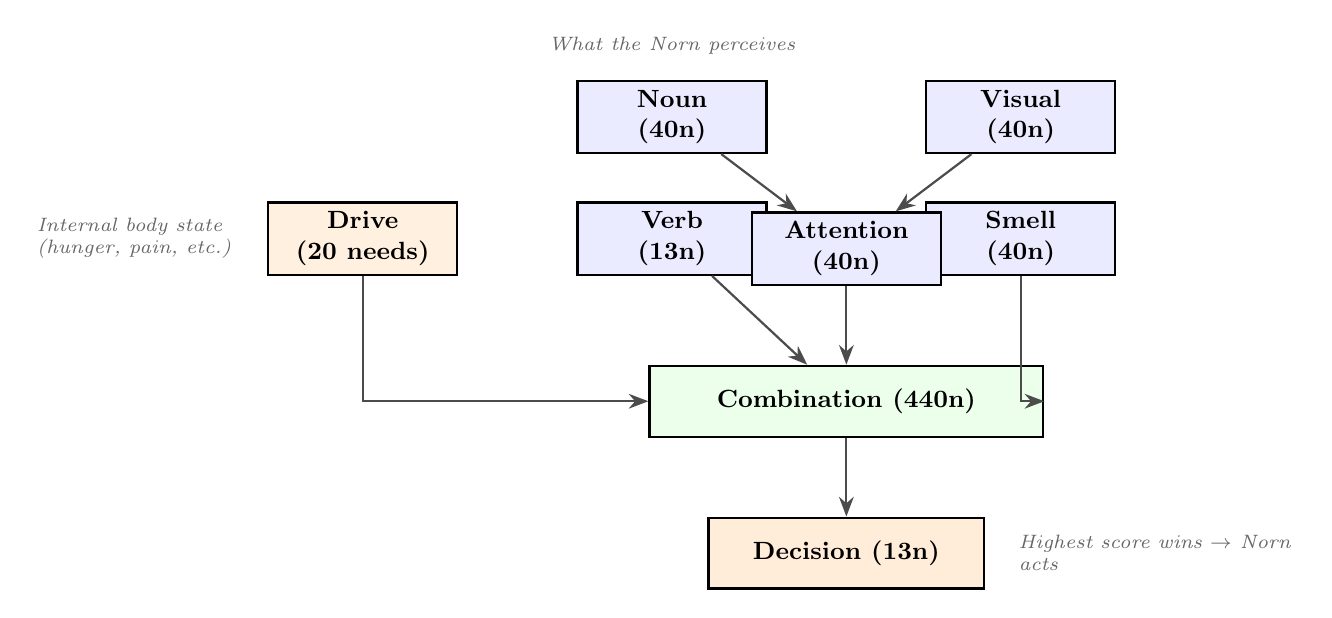
\begin{tikzpicture}[
    node distance=1.2cm and 1.8cm,
    lobe/.style={rectangle, draw=black, thick, fill=blue!8, minimum width=2.4cm, minimum height=0.9cm, align=center, font=\small\bfseries},
    lobekey/.style={rectangle, draw=black, thick, fill=orange!12, minimum width=2.4cm, minimum height=0.9cm, align=center, font=\small\bfseries},
    arrow/.style={-{Stealth[length=2.5mm]}, thick, draw=black!70},
    label/.style={font=\scriptsize\itshape, text=black!60},
  ]

  % Sensory input layer
  \node[lobe] (noun) {Noun\\(40n)};
  \node[lobe, right=2.0cm of noun] (visn) {Visual\\(40n)};
  \node[lobe, below=0.6cm of noun] (verb) {Verb\\(13n)};
  \node[lobe, right=2.0cm of verb] (smel) {Smell\\(40n)};

  % Attention
  \node[lobe, below=1.2cm of $(noun)!0.5!(visn)$] (attn) {Attention\\(40n)};

  % Drive
  \node[lobekey, left=1.5cm of verb] (drive) {Drive\\(20 needs)};

  % Processing
  \node[lobe, below=1.0cm of attn, minimum width=5cm, fill=green!8] (comb) {Combination (440n)};

  % Decision
  \node[lobekey, below=1.0cm of comb, minimum width=3.5cm, fill=orange!15] (decn) {Decision (13n)};

  % Arrows
  \draw[arrow] (noun) -- (attn);
  \draw[arrow] (visn) -- (attn);
  \draw[arrow] (attn) -- (comb);
  \draw[arrow] (drive) |- (comb);
  \draw[arrow] (verb) -- (comb);
  \draw[arrow] (smel) |- (comb);
  \draw[arrow] (comb) -- (decn);

  % Labels
  \node[above=0.2cm of noun, label] {What the Norn perceives};
  \node[right=0.3cm of decn, label, text width=3.5cm] {Highest score wins $\rightarrow$ Norn acts};
  \node[left=0.3cm of drive, label, text width=2.5cm] {Internal body state (hunger, pain, etc.)};

\end{tikzpicture}
\caption{\textbf{How a Norn's brain makes decisions (simplified).} Information flows top-to-bottom: sensory input (what the Norn sees, hears, and smells) enters at the top, combines with internal needs (hunger, pain, etc.) in the Combination lobe (the brain's largest region at 440 neurons), and converges on the Decision lobe where Winner-Takes-All competition selects a single action. Orange-highlighted lobes are the primary sites where our metabolic cost is applied. Not shown for clarity: Stimulus Source, Motor, Detail, Situation, Response, Friend-or-Foe, and Mood lobes (see Table~\ref{tab:lobes} for the complete 15-lobe architecture).}
\label{fig:brain-architecture}
\end{figure}

% ─── 3.3 Independent Variable: Metabolic Penalty ────────────────────────────
\subsection{Independent Variable: Metabolic Brain Cost}
\label{sec:iv}

The independent variable\footnote{In experimental science, the \emph{independent variable} is the thing the researcher deliberately changes to see what effect it has. The \emph{dependent variables} are the things that are measured to detect the effect.} is a binary treatment: \textbf{metabolic brain cost ON} (treatment group) vs.\ \textbf{metabolic brain cost OFF} (control group, the unmodified \textit{Creatures~3} game).

In the treatment condition, the following modifications are made at the C++ engine level:

\begin{description}[style=nextline, font=\itshape]
  \item[Synaptic Firing Cost --- ``Thinking Costs Energy'']
    On every engine tick, for every neuron in the Decision and Combination lobes whose activation exceeds a threshold $\theta_{\text{fire}} > 0$, a fixed amount $\delta_{\text{fire}}$ of ATP is deducted from the Norn's biochemistry:
    \begin{equation}
      \text{ATP}_{t+1} = \text{ATP}_t - \delta_{\text{fire}} \cdot |\{n \in \mathcal{L} : a_n(t) > \theta_{\text{fire}}\}|
      \label{eq:firing-cost}
    \end{equation}

    \begin{plainbox}
    Each tick, the engine counts how many neurons are actively firing in the key brain regions. For each firing neuron, a small amount of the creature's energy (ATP) is deducted. The more neurons firing at once, the more energy is consumed. A Norn that activates its entire brain simultaneously will drain its energy reserves faster than one that activates only the neurons it needs.
    \end{plainbox}

  \item[Synaptic Migration Penalty --- ``Rewiring Costs Energy'']
    When a synapse detaches from its post-synaptic neuron and migrates to a new target (a structural model update), an additional penalty $\delta_{\text{mig}}$ is deducted:
    \begin{equation}
      \text{ATP}_{t+1} = \text{ATP}_t - \delta_{\text{mig}} \cdot |\text{migrations at tick } t|
      \label{eq:migration-cost}
    \end{equation}

    \begin{plainbox}
    Every time a brain connection disconnects from one neuron and reattaches to another (``migration''), an extra energy cost is applied. This is like a moving fee---every time you rearrange your mental furniture, you pay a price. This discourages constant, aimless rewiring and favors stable, well-established connections.
    \end{plainbox}
\end{description}

\noindent The cost parameters $\delta_{\text{fire}}$ and $\delta_{\text{mig}}$ are \textbf{fixed runtime constants}, not genetically encoded traits. This means every Norn in the treatment group pays the same cost per brain operation---it is a universal environmental constraint (analogous to gravity) rather than something that can evolve. The values will be calibrated in pilot runs to be metabolically meaningful: large enough to noticeably affect ATP levels, but small enough that a well-fed Norn can sustain normal brain function.

\noindent\textbf{Rationale:} By modifying the engine at the C++ level rather than injecting chemicals via external scripting, we ensure that the metabolic deduction occurs synchronously within the brain's own update cycle, avoiding timing artifacts.

% ─── 3.4 Dependent Variables ─────────────────────────────────────────────────
\subsection{Dependent Variables: What We Measure}
\label{sec:dv}

We measure five quantities, three capturing brain efficiency and two capturing population-level survival:

\subsubsection{Biochemical State Entropy ($\Hbio$) --- ``How Chaotic Is the Body?''}
This metric measures how disordered the Norn's internal state is. It uses a standard information theory formula (Shannon entropy) applied to the 15 biological drive levels (Pain through Comfort, drives 0--14; the 5 navigational drives are excluded as they reflect spatial goals rather than homeostatic state):
\begin{equation}
  \Hbio = -\sum_{i=0}^{14} P(d_i) \log_2 P(d_i)
  \label{eq:Hbio}
\end{equation}

\begin{plainbox}
Imagine a dashboard with 15 gauges---Hunger for Protein, Hunger for Carbohydrate, Hunger for Fat, Pain, Tiredness, Fear, Comfort, and so on. If all gauges are fluctuating wildly and unpredictably, that's \textbf{high entropy} (disorder). If most gauges stay near comfortable levels with only small, predictable changes, that's \textbf{low entropy} (stability).

A healthy Norn should have low entropy: it eats when hungry, rests when tired, and keeps its internal chemistry balanced. A struggling Norn will have high entropy: its needs spike and crash erratically.
\end{plainbox}

\subsubsection{Synaptic Migration Rate ($\Rmig$) --- ``How Often Is the Brain Rewiring?''}
The rate of synaptic detachment and re-allocation across the brain's active connections:
\begin{equation}
  \Rmig = \frac{\Delta \text{Synapses Migrated}}{\Delta t}
  \label{eq:Rmig}
\end{equation}

\begin{plainbox}
This counts how many brain connections disconnect and reattach per unit of time. A high migration rate means the brain is constantly rearranging itself---it hasn't ``settled'' on what it knows. A low migration rate means the brain has found a stable configuration. We predict that metabolically constrained Norns will stabilize faster.
\end{plainbox}

\subsubsection{Bayesian Complexity Metric ($C$) --- ``How Much Has the Brain Changed From Birth?''}
The cumulative drift of synaptic weights from their initial (birth) values:
\begin{equation}
  C = \sum_{j} |w_j(t) - w_j(\text{birth})|
  \label{eq:complexity}
\end{equation}

\begin{plainbox}
Every Norn is born with a genetically determined set of brain connections (its ``blueprint''). Over its lifetime, learning changes the strengths of these connections. This metric measures the \emph{total amount of change} from the original blueprint. A high $C$ means the brain has been heavily remodeled; a low $C$ means it stayed close to its genetic starting point. Under metabolic constraints, we expect $C$ to plateau earlier and at a lower value---the brain makes the minimum necessary changes and then stops.
\end{plainbox}

\subsubsection{Time-to-Extinction ($T_{\text{ext}}$) --- ``How Long Does the Population Survive?''}
The total number of simulation ticks from trial start until the population reaches zero Norns. If the population survives to the maximum trial duration (3{,}000{,}000 ticks, $\approx$14 hours of simulated time), $T_{\text{ext}}$ is right-censored\footnote{In survival analysis, \emph{right-censoring} means we know the subject survived at least until the end of the observation period, but we don't know exactly how much longer it would have survived. It's like noting ``this patient was still alive when the study ended'' rather than ``this patient survived exactly X years.''} at that value.

\subsubsection{Population Trajectory ($N(t)$) --- ``How Does the Colony Size Change Over Time?''}
The number of living Norns at each snapshot interval, forming a time series $N(t)$ over the trial duration. We analyze mean population size, population variance (how much it fluctuates), and overall trend (growing, stable, or declining).

% ─── 3.5 Experimental Design ─────────────────────────────────────────────────
\subsection{Experimental Design}
\label{sec:design}

\begin{table}[H]
\centering
\caption{Experimental design summary. Each ``run'' is an independent simulation of a Norn colony from birth to extinction (or the maximum time limit).}
\label{tab:design}
\begin{tabular}{@{}ll@{}}
\toprule
\textbf{Parameter} & \textbf{Value} \\
\midrule
Design             & 2-condition between-subjects \\
Conditions         & Treatment (metabolic cost ON) vs.\ Control (cost OFF) \\
Replications       & $N = 10$ independent runs per condition \\
Initial population & 4 Norns (2 male, 2 female), identical base genome \\
Trial termination  & Population extinction ($N = 0$) or 3{,}000{,}000 ticks \\
Snapshot interval  & Every 1{,}000 ticks \\
Execution mode     & Headless, 100$\times$ speed \\
Total runs         & 20 \\
\bottomrule
\end{tabular}
\end{table}

\begin{plainbox}
\textbf{The experimental setup in everyday terms:} We run 20 separate ``colonies'' of virtual creatures---10 where brain activity costs energy and 10 where it doesn't. Each colony starts with exactly the same 4 creatures (2 males and 2 females from the same genetic template). We then let each colony run on its own, with no human intervention, until either all creatures die or 14 hours of simulated time passes. Every few seconds of game time, we take a detailed ``medical scan'' of every creature---recording their brain activity, body chemistry, and vital signs---and save it for later analysis.

\medskip
Because the simulation involves random elements (mutations during reproduction, random brain initialization), no two runs are exactly alike even with the same starting conditions. This randomness is why we repeat each condition 10 times: to distinguish real effects from coincidence.
\end{plainbox}

\noindent\textbf{Randomization:} Each run uses a fresh world. The 4 initial Norns are hatched from the same base genome with specified sex assignments. Stochasticity arises from the engine's internal random number generator (seeded differently per run), which affects biochemistry update order, mutation during reproduction, and neural initialization noise.

\noindent\textbf{Controlled variables:} Environment layout, food distribution, object placement, and all game bootstrap scripts are identical across all runs. No player interaction occurs during headless execution.

\noindent\textbf{Pre-registration commitment:} Prior to data collection, the final protocol---including calibrated values for $\delta_{\text{fire}}$ and $\delta_{\text{mig}}$---will be deposited as a formal pre-registration on the Open Science Framework (OSF, \url{https://osf.io}). This ensures that the hypotheses, experimental design, and analysis plan are timestamped and publicly frozen before any results are observed, protecting against post-hoc modification of the protocol.

% ═════════════════════════════════════════════════════════════════════════════
\section{Protocol}
\label{sec:protocol}

% ─── Protocol Flowchart ─────────────────────────────────────────────────────
\begin{figure}[H]
\centering
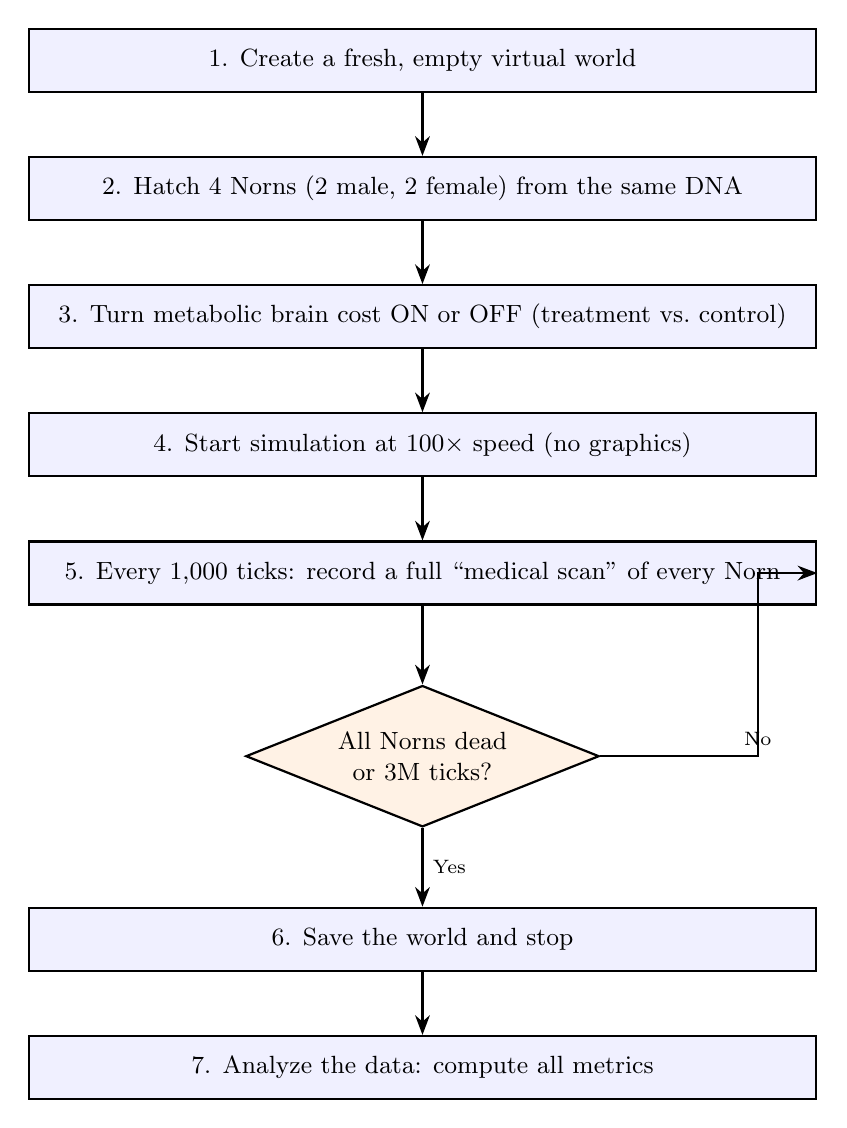
\begin{tikzpicture}[
    node distance=0.8cm,
    pstep/.style={rectangle, draw=black, thick, fill=blue!6, minimum width=10cm, minimum height=0.8cm, align=center, font=\small},
    decision/.style={diamond, draw=black, thick, fill=orange!10, minimum width=2.5cm, align=center, font=\small, aspect=2.5},
    arrow/.style={-{Stealth[length=2.5mm]}, thick},
  ]

  \node[pstep] (s1) {1. Create a fresh, empty virtual world};
  \node[pstep, below=of s1] (s2) {2. Hatch 4 Norns (2 male, 2 female) from the same DNA};
  \node[pstep, below=of s2] (s3) {3. Turn metabolic brain cost ON or OFF (treatment vs.\ control)};
  \node[pstep, below=of s3] (s4) {4. Start simulation at 100$\times$ speed (no graphics)};
  \node[pstep, below=of s4] (s5) {5. Every 1{,}000 ticks: record a full ``medical scan'' of every Norn};
  \node[decision, below=1.0cm of s5] (d1) {All Norns dead\\or 3M ticks?};
  \node[pstep, below=1.0cm of d1] (s6) {6. Save the world and stop};
  \node[pstep, below=of s6] (s7) {7. Analyze the data: compute all metrics};

  \draw[arrow] (s1) -- (s2);
  \draw[arrow] (s2) -- (s3);
  \draw[arrow] (s3) -- (s4);
  \draw[arrow] (s4) -- (s5);
  \draw[arrow] (s5) -- (d1);
  \draw[arrow] (d1) -- node[right, font=\scriptsize] {Yes} (s6);
  \draw[arrow] (d1.east) -- ++(2,0) node[above, font=\scriptsize] {No} |- (s5.east);
  \draw[arrow] (s6) -- (s7);

\end{tikzpicture}
\caption{\textbf{What happens in each trial.} The protocol is fully automated: no human intervenes once the simulation starts. The loop in steps 5--6 continues recording data until the colony goes extinct or the time limit is reached.}
\label{fig:protocol}
\end{figure}

\subsection{Detailed Protocol Steps}

\begin{enumerate}
  \item \textbf{World Creation.} A fresh, empty world is created using the engine's API. This ensures no leftover state from previous runs---each trial is truly independent.

  \item \textbf{Population Seeding.} Four Norns are hatched from the same base genome template: 2 males and 2 females. This gives the colony reproductive potential while keeping initial conditions identical across all 20 runs.

  \item \textbf{Condition Assignment.} For treatment runs, the engine's metabolic brain cost is switched on (a runtime flag). For control runs, it stays off. The cost parameters ($\delta_{\text{fire}}$ and $\delta_{\text{mig}}$) are set to values determined during pilot calibration.

  \item \textbf{Simulation Execution.} The engine runs in headless mode at 100$\times$ speed. A bootstrap script configures the data collection pipeline to record snapshots every 1{,}000 ticks.

  \item \textbf{Telemetry Snapshots.} Each snapshot records, for every living Norn:
    \begin{itemize}[nosep]
      \item Current tick number (timestamp).
      \item All 20 drive levels (three kinds of hunger, pain, tiredness, fear, etc.).
      \item All 256 chemical concentrations in the bloodstream.
      \item Organ health status.
      \item Brain lobe activity---which neurons are firing and how strongly.
      \item Current synaptic weight values (connection strengths).
      \item Number of synaptic migrations since the last snapshot.
    \end{itemize}

  \item \textbf{Termination.} The trial ends when the population reaches zero (all Norns have died) or the tick count exceeds 3{,}000{,}000 ($\approx$14 hours of simulated time, covering 2--3 full Norn lifetimes). The world state is saved to disk.

  \item \textbf{Post-Processing.} Python scripts compute the five metrics ($\Hbio$, $\Rmig$, $C$, $T_{\text{ext}}$, $N(t)$) from the saved snapshots. All analysis code will be published alongside the engine source.
\end{enumerate}

% ═════════════════════════════════════════════════════════════════════════════
\section{Analysis Plan}
\label{sec:analysis}

\subsection{Primary Confirmatory Analysis}

All between-group comparisons use two-sided \textbf{Mann-Whitney~U tests}\footnote{The Mann-Whitney U test is a statistical test that compares two groups without assuming their data follow a bell curve. It asks: ``Are the values in Group A consistently higher (or lower) than in Group B?'' It is robust for small samples (like our N=10 per group).}. We test:

\begin{table}[H]
\centering
\caption{Primary confirmatory tests. All tests are two-sided with $\alpha = 0.05$ (the standard threshold: we consider a result ``statistically significant'' if there is less than a 5\% probability it occurred by chance).}
\label{tab:tests}
\begin{tabular}{@{}llll@{}}
\toprule
\textbf{Hypothesis} & \textbf{What We Measure} & \textbf{Predicted Direction} & \textbf{Plain Meaning} \\
\midrule
H1.1(i)   & Migration rate ($\Rmig$)        & Treatment $<$ Control & Less rewiring \\
H1.1(ii)  & Brain change ($C$)              & Treatment $<$ Control & Less change from blueprint \\
H1.2(i)   & Survival time ($T_{\text{ext}}$) & Treatment $>$ Control & Longer survival \\
H1.2(ii)  & Body chaos ($\Hbio$)            & Treatment $<$ Control & More stable body chemistry \\
H1.2(iii) & Pop.\ variance                  & Treatment $<$ Control & More stable colony size \\
\bottomrule
\end{tabular}
\end{table}

\noindent For time-to-extinction, we also plot \textbf{Kaplan-Meier survival curves}\footnote{A Kaplan-Meier curve is a step-function graph commonly used in medical research to show the fraction of a population surviving over time. It visually answers the question ``What percentage of colonies are still alive at each point in time?''}---a standard tool from medical research that visually shows how the two groups' survival compares over time.

\subsection{Supplementary Bayesian Analysis}

As a planned supplementary analysis, we compute \textbf{Bayes factors} ($\text{BF}_{10}$) for each hypothesis. Unlike the Mann-Whitney test, which simply asks ``is there a statistically significant difference?'', the Bayes factor asks \emph{``how much more likely are the data under our hypothesis than under the null (no-effect) hypothesis?''}

\begin{plainbox}
A Bayes factor of 1 means both hypotheses are equally likely given the data. A Bayes factor of 10 means our hypothesis is 10 times more likely than ``no effect.'' We use this as a supplementary analysis because it provides a nuanced, continuous measure of evidence rather than a simple yes/no answer. It is also thematically fitting: we are studying Bayesian brains, so we analyze them with Bayesian statistics.
\end{plainbox}

\subsection{Exploratory Analyses}

The following analyses are declared as exploratory (not bound by the confirmatory protocol) and will be reported separately:
\begin{itemize}[nosep]
  \item How do brain chaos ($\Hbio$) and rewiring rate ($\Rmig$) change over time? Do they converge?
  \item Do individual Norns that consume less ATP per tick live longer?
  \item Do the two groups have differently shaped distributions of connection strengths?
  \item How many generations of offspring does each colony produce before extinction?
\end{itemize}

% ═════════════════════════════════════════════════════════════════════════════
\section{System Architecture}
\label{sec:architecture}

% ─── System Architecture Diagram ─────────────────────────────────────────────
\begin{figure}[H]
\centering
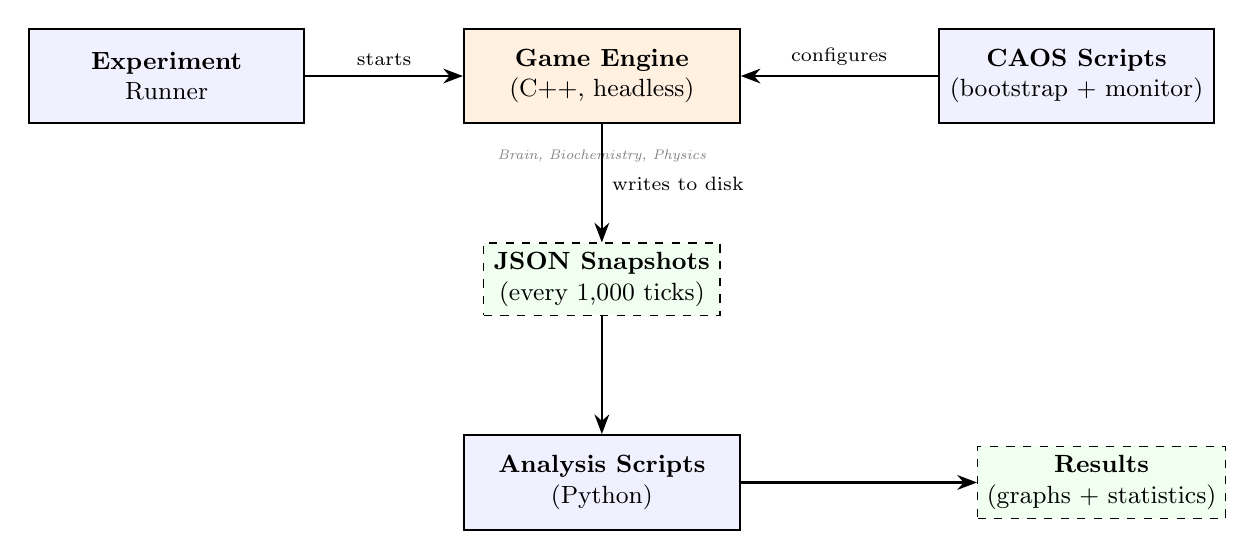
\begin{tikzpicture}[
    node distance=1.0cm and 2.0cm,
    block/.style={rectangle, draw=black, thick, fill=blue!6, minimum width=3.5cm, minimum height=1.2cm, align=center, font=\small},
    blockkey/.style={rectangle, draw=black, thick, fill=orange!12, minimum width=3.5cm, minimum height=1.2cm, align=center, font=\small},
    data/.style={rectangle, draw=black, dashed, fill=green!6, minimum width=3.0cm, minimum height=0.9cm, align=center, font=\small},
    arrow/.style={-{Stealth[length=2.5mm]}, thick},
    darrow/.style={-{Stealth[length=2.5mm]}, thick, dashed},
  ]

  % Engine
  \node[blockkey] (engine) {\textbf{Game Engine}\\(C++, headless)};
  \node[below=0.2cm of engine, font=\tiny\itshape, text=black!50] {Brain, Biochemistry, Physics};

  % Telemetry
  \node[data, below=1.5cm of engine] (json) {\textbf{JSON Snapshots}\\(every 1{,}000 ticks)};

  % Analysis
  \node[block, below=1.5cm of json] (python) {\textbf{Analysis Scripts}\\(Python)};

  % Results
  \node[data, right=3.0cm of python] (results) {\textbf{Results}\\(graphs + statistics)};

  % Runner
  \node[block, left=2.0cm of engine] (runner) {\textbf{Experiment}\\Runner};

  % CAOS
  \node[block, right=2.5cm of engine] (caos) {\textbf{CAOS Scripts}\\(bootstrap + monitor)};

  % Arrows
  \draw[arrow] (runner) -- node[above, font=\scriptsize] {starts} (engine);
  \draw[arrow] (caos) -- node[above, font=\scriptsize] {configures} (engine);
  \draw[arrow] (engine) -- node[right, font=\scriptsize] {writes to disk} (json);
  \draw[arrow] (json) -- (python);
  \draw[arrow] (python) -- (results);

\end{tikzpicture}
\caption{\textbf{How the experiment runs automatically.} The experiment runner script launches the game engine in headless mode. CAOS bootstrap scripts configure the initial population and telemetry settings. The engine natively writes JSON data snapshots to disk every 1{,}000 ticks. After all 20 runs are complete, Python scripts process the snapshots into statistical results and graphs. No external APIs or servers are required during experiment execution.}
\label{fig:architecture}
\end{figure}

% ═════════════════════════════════════════════════════════════════════════════
\section{Scope and Limitations}
\label{sec:limitations}

No experiment is without boundaries. We explicitly acknowledge the following:

\begin{enumerate}[label=(\alph*)]
  \item \textbf{Social communication is not tested here.} This proposal covers only internal brain metabolism (Layer~1). A follow-up experiment (Layer~2) will explore what happens when \emph{talking} also costs energy---testing whether metabolically expensive communication leads to more efficient language.

  \item \textbf{The energy cost cannot evolve.} In this experiment, the metabolic cost of brain activity is the same for all Norns and does not change across generations. Future work may explore whether Norns can \emph{evolve} different levels of metabolic efficiency, with more efficient brains conferring a survival advantage that is passed to offspring.

  \item \textbf{The brain is small.} The Creatures~3 brain has 815 neurons and 15 lobes---vastly smaller than a biological brain (86 billion neurons) or a large AI model (billions of parameters). Our results demonstrate the \emph{principle} of metabolic grounding; whether the effect scales to larger architectures remains an open question.

  \item \textbf{The environment is fixed.} All trials run in the standard Docking Station environment---a deliberately constrained habitat chosen over the larger Creatures~3 Shee Ark to minimize spatial confounds. We do not vary food scarcity, introduce predators, or change seasonal conditions. Testing the metabolic brain cost under varying environmental pressures is deferred to future experiments.

  \item \textbf{The game requires proprietary data.} While the engine source code is fully open, running the experiment requires game data files from \textit{Creatures Exodus} (available for purchase on Steam or GOG for approximately \$6). All novel code, analysis scripts, and results will be fully open-sourced.
\end{enumerate}

% ═════════════════════════════════════════════════════════════════════════════
\section{Expected Outcomes and Significance}
\label{sec:significance}

\subsection{If the Hypotheses Are Supported}

If \textbf{H1.1} is supported (brains become leaner), this experiment provides empirical evidence that \textbf{metabolic costs can replace abstract mathematical regularization} in neural networks. The FEP's complexity penalty---typically a term in an equation---would be shown to emerge naturally from the physical constraints of the substrate. The brain doesn't need an external ``penalty function''---it just needs to pay for its own operations.

If \textbf{H1.2} is supported (constrained creatures survive longer), the implications are more provocative. It would suggest that metabolic constraints are not merely a biological inconvenience to be engineered around, but a \textbf{computational advantage}: agents that pay a physical price for neural complexity are \emph{forced} to develop efficient representations, and this efficiency translates to superior survival.

\begin{analogybox}
This is similar to the ``paradox of constraints'' in engineering: a bridge that must be light (due to material limits) is often stronger than a bridge built with unlimited materials, because the constraint forces the engineer to find structurally optimal designs. We hypothesize that the metabolic constraint on brains works the same way.
\end{analogybox}

\subsection{If the Hypotheses Are Not Supported}

Even negative results would be valuable. They would suggest that either:
\begin{itemize}[nosep]
  \item the Creatures~3 brain is too small for the FEP's complexity-accuracy tradeoff to manifest,
  \item the metabolic costs we chose are too small (or too large) to produce measurable effects, or
  \item the FEP's complexity penalty fundamentally requires an information-theoretic (rather than metabolic) implementation.
\end{itemize}
Any of these findings would inform the design of future experiments with richer neural substrates.

\subsection{Broader Implications for AI}

The AI industry currently faces an energy crisis: training state-of-the-art models requires enormous computational resources and produces significant carbon emissions. If metabolic constraints can produce more efficient neural architectures---even in a simple system like Creatures~3---this opens a new design paradigm: building AI systems that are \emph{energy-aware by design}, not just energy-optimized as an afterthought.

% ═════════════════════════════════════════════════════════════════════════════
\section*{Supplementary Material}
\label{sec:supplementary}

The following resources provide additional context and full access to the experimental platform:

\begin{itemize}[nosep]
  \item \textbf{Engine source code:} \url{https://github.com/cyrilsadovsky/creatures3-engine-port}
  \item \textbf{Video --- AI Learning in Real Time (the ``limbic gap'' argument):}\\
    \url{https://www.youtube.com/watch?v=LyVzUs_rTQ4}
  \item \textbf{Video --- 1997 Creatures Paper Breakdown (the biology behind Norns):}\\
    \url{https://www.youtube.com/watch?v=Ymm6pWf1W0Q}
  \item \textbf{Video --- AI reads AI (AI-assisted engine exploration via MCP):}\\
    \url{https://www.youtube.com/watch?v=vz_2FZQ_2V8}
\end{itemize}

% ═════════════════════════════════════════════════════════════════════════════
\appendix
\section{Engineering Requirements}
\label{app:engineering}

This appendix maps each experimental requirement to the specific code and tool modifications needed, serving as a functional specification for the engineering work that must precede the experiment.

\subsection{C++ Engine Modifications}

\begin{table}[H]
\centering
\caption{Required engine-level modifications. These are changes to the game's C++ source code.}
\label{tab:engine-mods}
\begin{tabular}{@{}p{3.5cm}p{4cm}p{5.5cm}@{}}
\toprule
\textbf{What We Need} & \textbf{Where in the Code} & \textbf{What It Does} \\
\midrule
Synaptic firing cost & \texttt{Brain.cpp}, \texttt{Lobe.cpp} & Count active neurons each tick; deduct ATP per firing \\
Migration penalty & \texttt{Brain.cpp} & Detect synapse migrations; deduct ATP per migration \\
Migration counter & \texttt{Brain.cpp} & Track how many migrations occur, expose via API \\
Runtime toggle & \texttt{SDL\_Main.cpp} & Command-line flag to enable/disable metabolic cost \\
Snapshot writer & \texttt{DebugServer.cpp} & Automatic data dump every $N$ ticks \\
\bottomrule
\end{tabular}
\end{table}

\subsection{Automation Scripts}

\begin{itemize}[nosep]
  \item \textbf{Bootstrap script} (\texttt{fep\_experiment\_bootstrap.cos}): runs at world start; hatches 4 Norns and configures experiment parameters.
  \item \textbf{Snapshot timer}: triggers a data dump every 1{,}000 ticks.
  \item \textbf{Extinction monitor}: detects when all Norns have died and triggers a clean shutdown.
\end{itemize}

\subsection{Python Analysis Pipeline}

\begin{itemize}[nosep]
  \item \texttt{compute\_entropy.py}: calculates body chaos metric ($\Hbio$) from drive levels.
  \item \texttt{compute\_migration.py}: calculates rewiring rate ($\Rmig$) from migration counts.
  \item \texttt{compute\_complexity.py}: calculates brain change metric ($C$) from synaptic weights.
  \item \texttt{survival\_analysis.py}: generates survival curves and runs statistical tests.
  \item \texttt{statistical\_tests.py}: runs Mann-Whitney U tests and computes Bayes factors.
  \item \texttt{plot\_results.py}: generates publication-quality figures.
\end{itemize}

\subsection{Experiment Runner}

A shell script (\texttt{run\_experiment.sh}) that:
\begin{enumerate}[nosep]
  \item Runs 20 trials in sequence (10 treatment, 10 control).
  \item Creates a fresh world for each trial.
  \item Launches the engine in headless mode with the appropriate flags.
  \item Monitors for termination (all Norns dead, or maximum ticks reached).
  \item Organizes output into numbered directories for analysis.
\end{enumerate}

% ═════════════════════════════════════════════════════════════════════════════
\bibliographystyle{plainnat}
\bibliography{references}

\end{document}
